\documentclass[aspectratio=169,11pt]{beamer}

\usepackage[T1]{fontenc}
\usepackage{lmodern}
\usepackage{graphicx}
\usepackage{booktabs}
\usepackage{tikz}
\usetikzlibrary{positioning,arrows.meta}

\graphicspath{{figures/}}

% ---- Look and feel -------------------------------------------------------------------------------
\definecolor{sentry}{RGB}{16,60,54}
\definecolor{alertred}{RGB}{183,39,33}
\definecolor{soft}{RGB}{244,241,234}
\setbeamercolor{frametitle}{fg=sentry}
\setbeamercolor{title}{fg=sentry}
\setbeamercolor{structure}{fg=sentry}
\setbeamercolor{background canvas}{bg=white}
\setbeamerfont{frametitle}{series=\bfseries,size=\Large}
\setbeamertemplate{navigation symbols}{}
\setbeamertemplate{itemize items}[circle]
\setbeamertemplate{footline}{\hfill\color{gray}\scriptsize\insertframenumber\,/\,\inserttotalframenumber\hspace{1em}\vspace{0.6em}}
\newcommand{\bignum}[1]{{\Huge\bfseries\color{sentry}#1}}

\title{SentryCare}
\subtitle{AI camera monitoring for resident safety in aged care}
\author{Kaushalendra Pratap Singh \and Dhruv Jain \and Nandish Bhatt \and Dev Upadhyay}
\date{}

\begin{document}

% 1 ---------------------------------------------------------------------------------------------
\begin{frame}[plain]
\begin{tikzpicture}[remember picture,overlay]
  \fill[sentry] (current page.north west) rectangle ([yshift=-0.25cm]current page.north east);
\end{tikzpicture}
\vfill
\centering
{\fontsize{40}{44}\selectfont\bfseries\color{sentry} SentryCare}\\[0.6em]
{\Large AI camera monitoring for resident safety in aged care}\\[2.2em]
\small
\begin{tabular}{cccc}
Kaushalendra Pratap Singh & Dhruv Jain & Nandish Bhatt & Dev Upadhyay\\
AU2644013 & AU2644029 & AU2644012 & AU2644003
\end{tabular}\\[1.8em]
{\color{gray}\footnotesize Project Track: Application Based}
\vfill
\end{frame}

% 2 ---------------------------------------------------------------------------------------------
\begin{frame}{The problem}
\begin{columns}[c]
\column{0.5\textwidth}
\centering
\bignum{Cameras record.}\\[0.4em]
\bignum{Nobody watches.}
\column{0.5\textwidth}
\begin{itemize}\setlength\itemsep{1.2em}
  \item Falls are a major risk for older adults
  \item Help is late if no one sees the fall
  \item Wearable sensors are often forgotten or removed
  \item Care homes already have cameras: \textbf{use them}
\end{itemize}
\end{columns}
\end{frame}

% 3 ---------------------------------------------------------------------------------------------
\begin{frame}{Objectives}
\centering
\resizebox{\linewidth}{!}{%
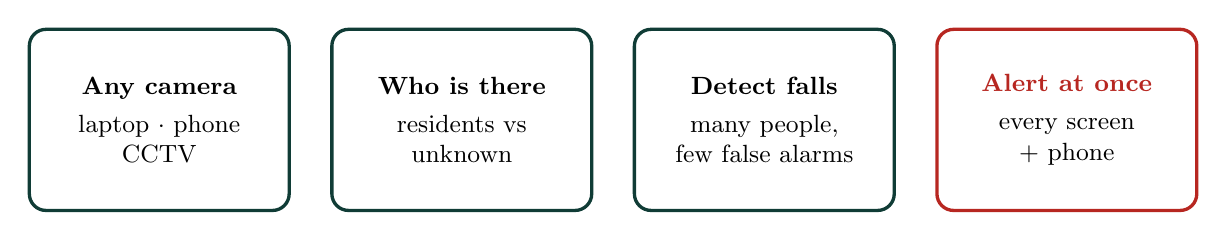
\begin{tikzpicture}[box/.style={draw=sentry, very thick, rounded corners=6pt, minimum width=3.3cm,
                    minimum height=2.3cm, align=center, font=\small}]
  \node[box] (a) {\textbf{Any camera}\\[0.3em] laptop $\cdot$ phone\\ CCTV};
  \node[box, right=0.5cm of a] (b) {\textbf{Who is there}\\[0.3em] residents vs\\ unknown};
  \node[box, right=0.5cm of b] (c) {\textbf{Detect falls}\\[0.3em] many people,\\ few false alarms};
  \node[box, right=0.5cm of c, draw=alertred] (d) {\textcolor{alertred}{\textbf{Alert at once}}\\[0.3em] every screen\\ + phone};
\end{tikzpicture}%
}\\[2em]
\large Runs on an ordinary laptop \quad$\cdot$\quad personal data stays on the computer
\end{frame}

% 4 ---------------------------------------------------------------------------------------------
\begin{frame}{System architecture}
\centering
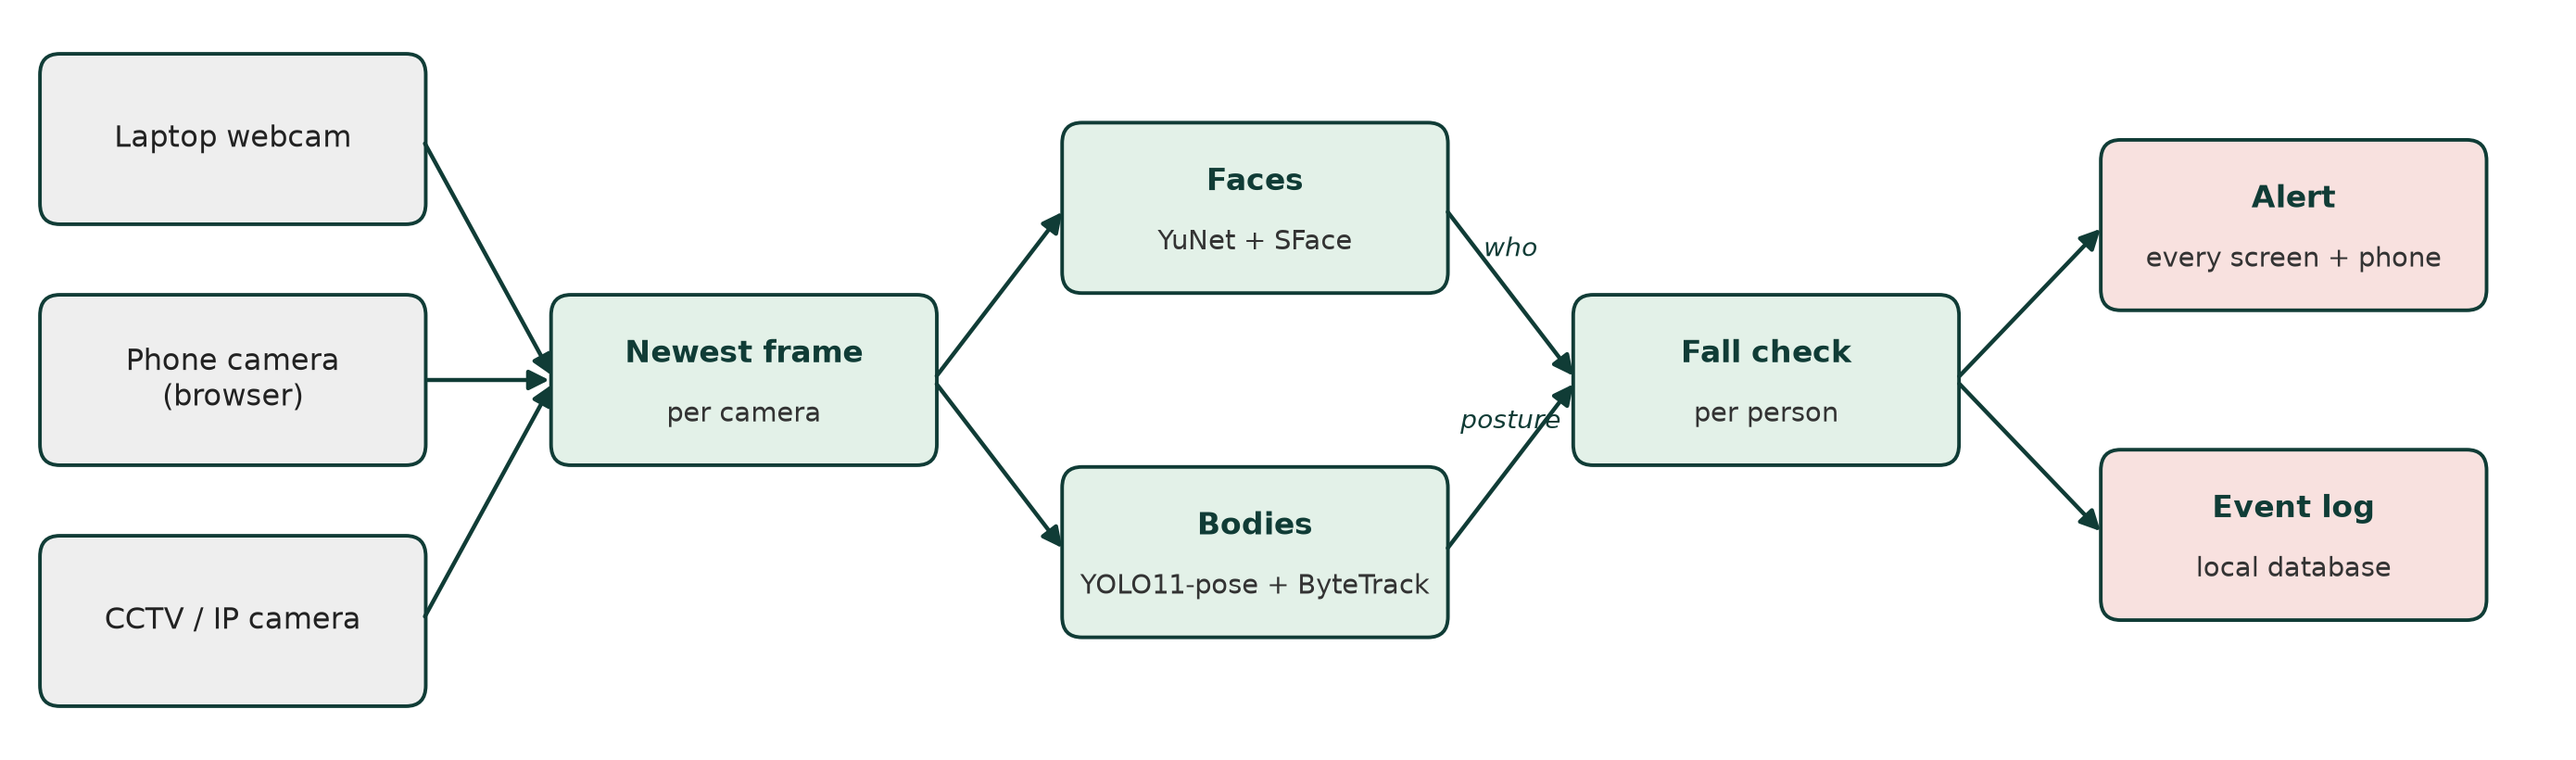
\includegraphics[width=\linewidth]{architecture.png}\\[1.2em]
\small Everything runs locally on one laptop CPU
\end{frame}

% 5 ---------------------------------------------------------------------------------------------
\begin{frame}{Recognising faces}
\begin{columns}[c]
\column{0.42\textwidth}
\begin{enumerate}\setlength\itemsep{0.9em}
  \item \textbf{Find} the face
  \item \textbf{Align} it the same way
  \item Turn it into \textbf{128 numbers}
  \item \textbf{Compare} with enrolled people
\end{enumerate}
\vspace{1em}
Score $\geq$ 0.45 $\Rightarrow$ name\\
otherwise $\Rightarrow$ \textbf{Unknown}
\column{0.58\textwidth}
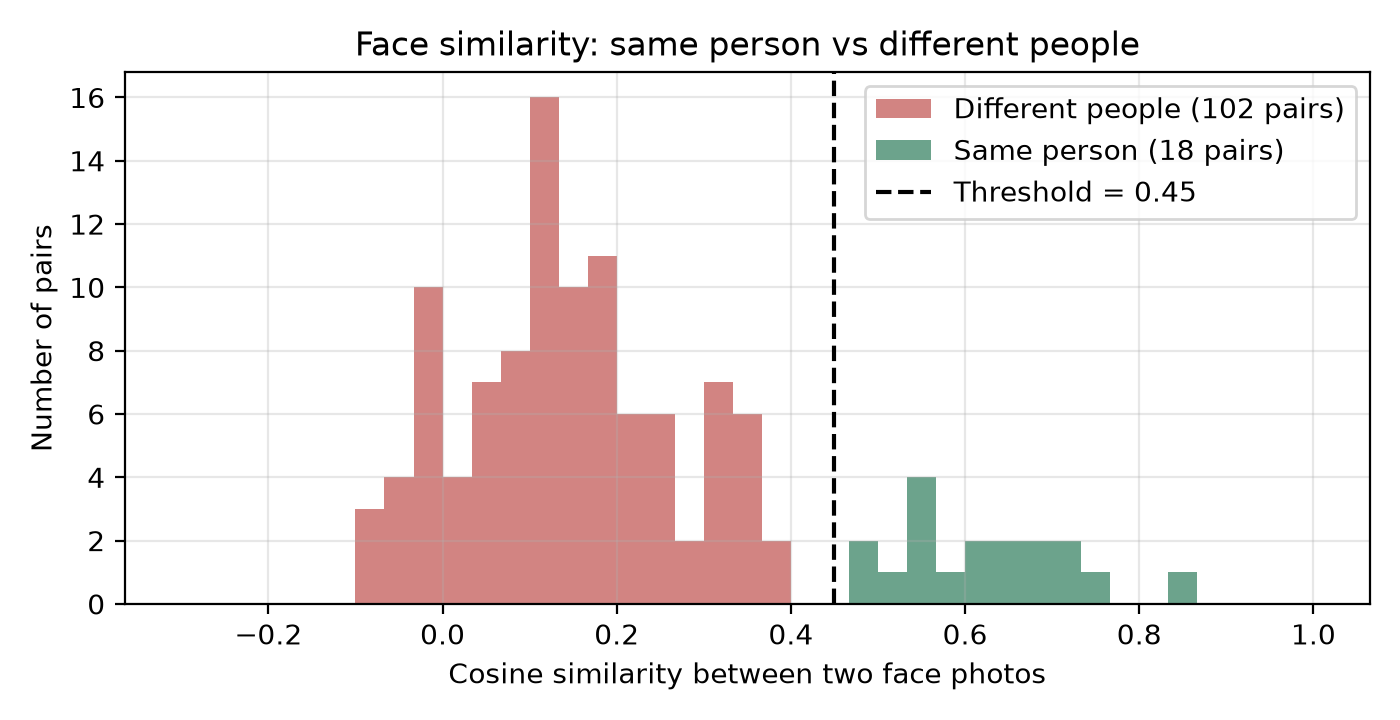
\includegraphics[width=\linewidth]{face_similarity.png}
\end{columns}
\end{frame}

% 6 ---------------------------------------------------------------------------------------------
\begin{frame}{Detecting falls}
\centering
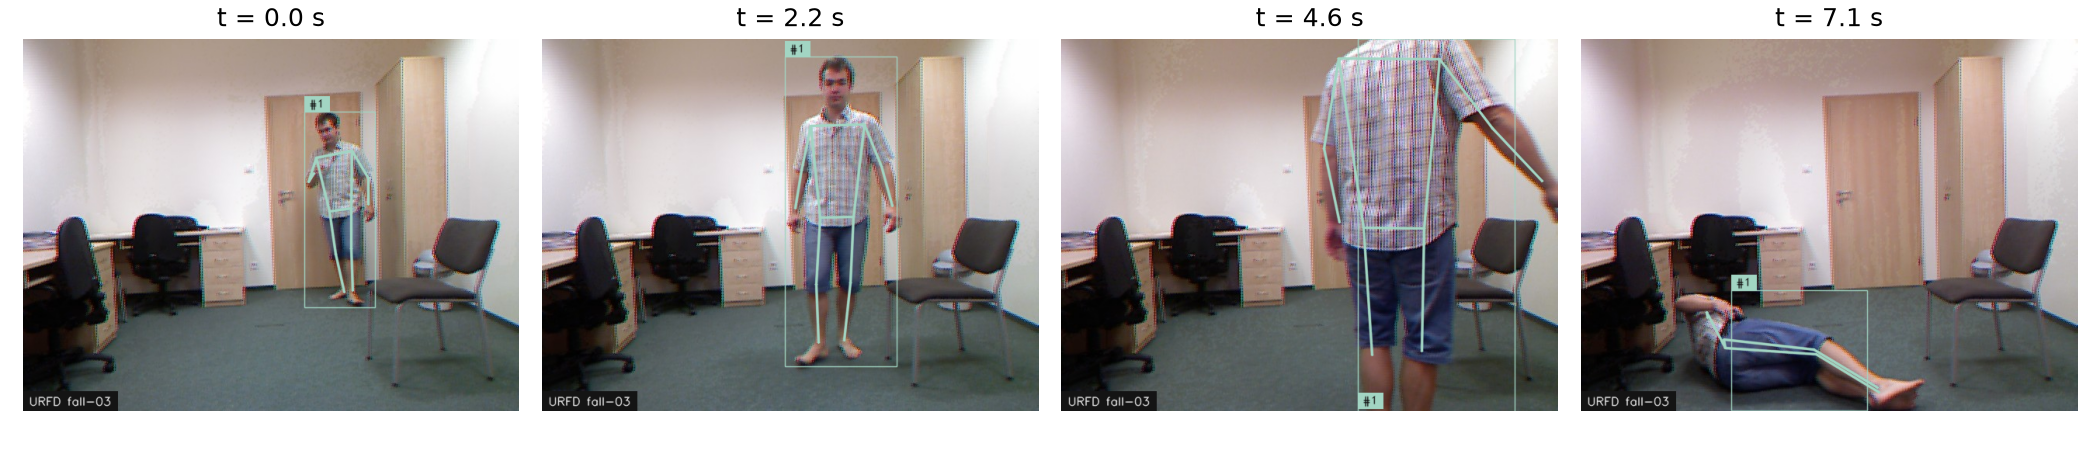
\includegraphics[width=\linewidth]{fall_sequence.png}\\[0.8em]
\begin{columns}[t]
\column{0.32\textwidth}\centering \textbf{Track everyone}\\ \small each person, own fall check
\column{0.32\textwidth}\centering \textbf{Confirm it}\\ \small down 1.2~s, stays down 2~s
\column{0.32\textwidth}\centering \textbf{Don't lose them}\\ \small box continuation + track hand-off
\end{columns}
\vfill\hfill{\tiny\color{gray} Images: UR Fall Detection dataset (Kwolek \& Kepski, 2014), CC BY-NC-SA 4.0}
\end{frame}

% 7 ---------------------------------------------------------------------------------------------
\begin{frame}{Cameras and alerts}
\begin{columns}[c]
\column{0.62\textwidth}
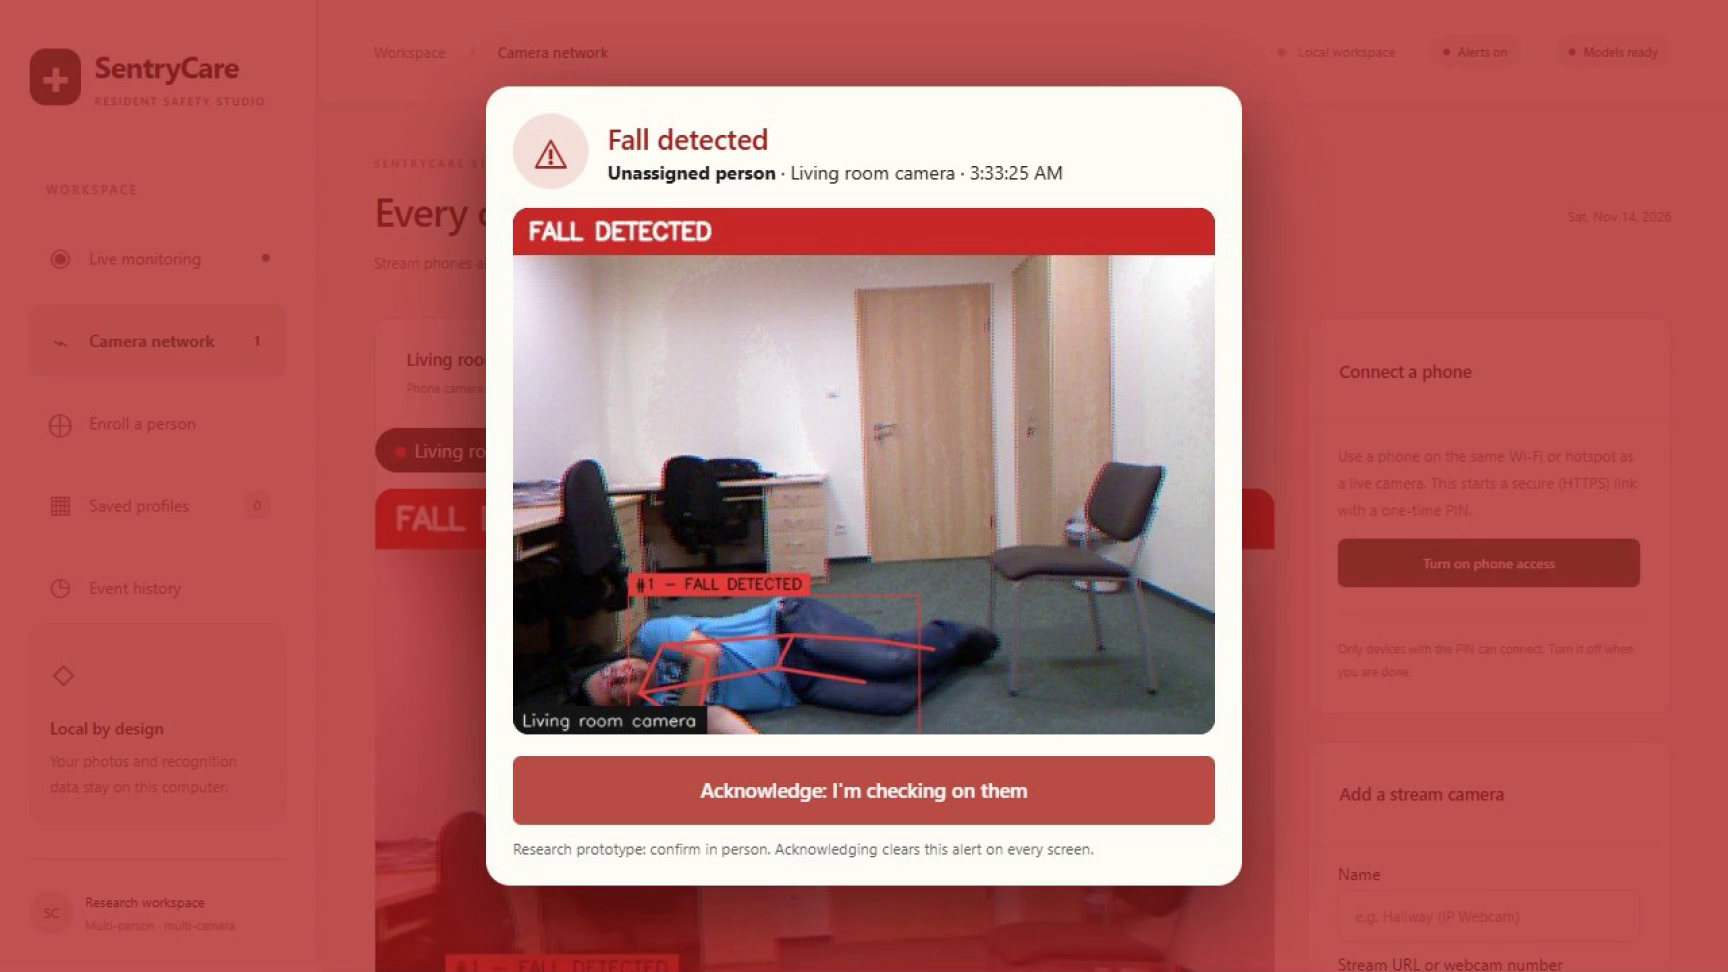
\includegraphics[width=\linewidth]{dashboard_alert.png}
\column{0.38\textwidth}
\begin{itemize}\setlength\itemsep{1em}
  \item Phone = camera\\ \small scan a QR code, enter PIN
  \item Alarm on \textbf{every} screen\\ \small snapshot + siren
  \item One tap to \textbf{acknowledge}
  \item Optional phone push
\end{itemize}
\end{columns}
\vfill\hfill{\tiny\color{gray} Images: UR Fall Detection dataset (Kwolek \& Kepski, 2014), CC BY-NC-SA 4.0}
\end{frame}

% 8 ---------------------------------------------------------------------------------------------
\begin{frame}{Experiments}
\begin{columns}[c]
\column{0.5\textwidth}
\textbf{UR Fall Detection dataset}\\[0.5em]
\begin{tabular}{lcc}
\toprule
 & Falls & Normal activity \\
\midrule
Test videos & 13 & 13 \\
Development & 2 & 2 \\
\bottomrule
\end{tabular}\\[1.2em]
\textbf{Faces:} 5 enrolled people, 16 photos
\column{0.5\textwidth}
\begin{itemize}\setlength\itemsep{1em}
  \item Same speed as live: \textbf{5 frames / s}
  \item Old vs new pipeline, same videos
  \item Measure: falls caught, false alarms, delay
  \item Switch off one rule at a time
\end{itemize}
\end{columns}
\end{frame}

% 9 ---------------------------------------------------------------------------------------------
\begin{frame}{Results}
\begin{columns}[c]
\column{0.58\textwidth}
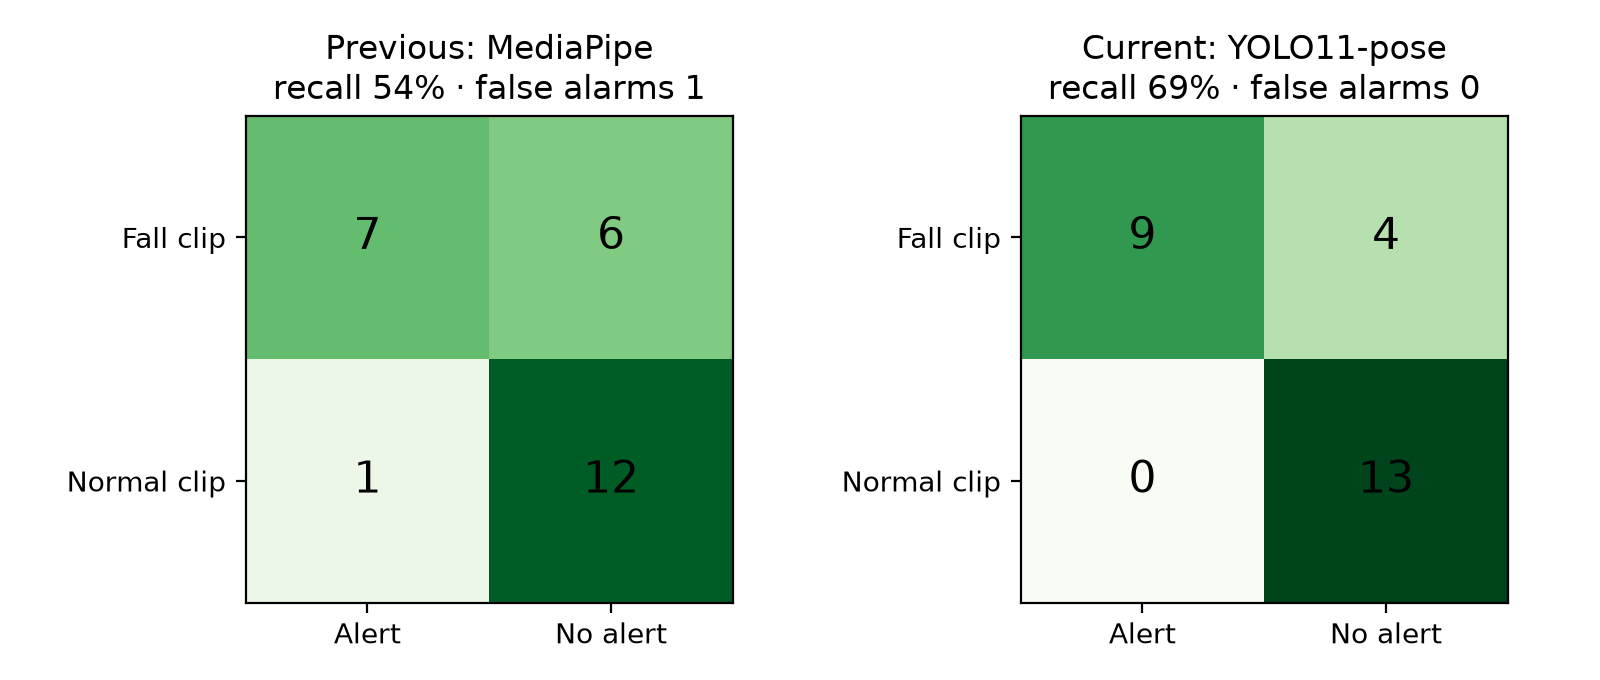
\includegraphics[width=\linewidth]{fall_confusion.png}
\column{0.42\textwidth}
\centering
\bignum{9 / 13} \\ \small falls caught (was 7)\\[1.2em]
\bignum{0 / 13} \\ \small false alarms (was 1)\\[1.2em]
\bignum{16 / 16} \\ \small faces identified correctly
\end{columns}
\end{frame}

% 10 --------------------------------------------------------------------------------------------
\begin{frame}{Analysis}
\begin{columns}[c]
\column{0.6\textwidth}
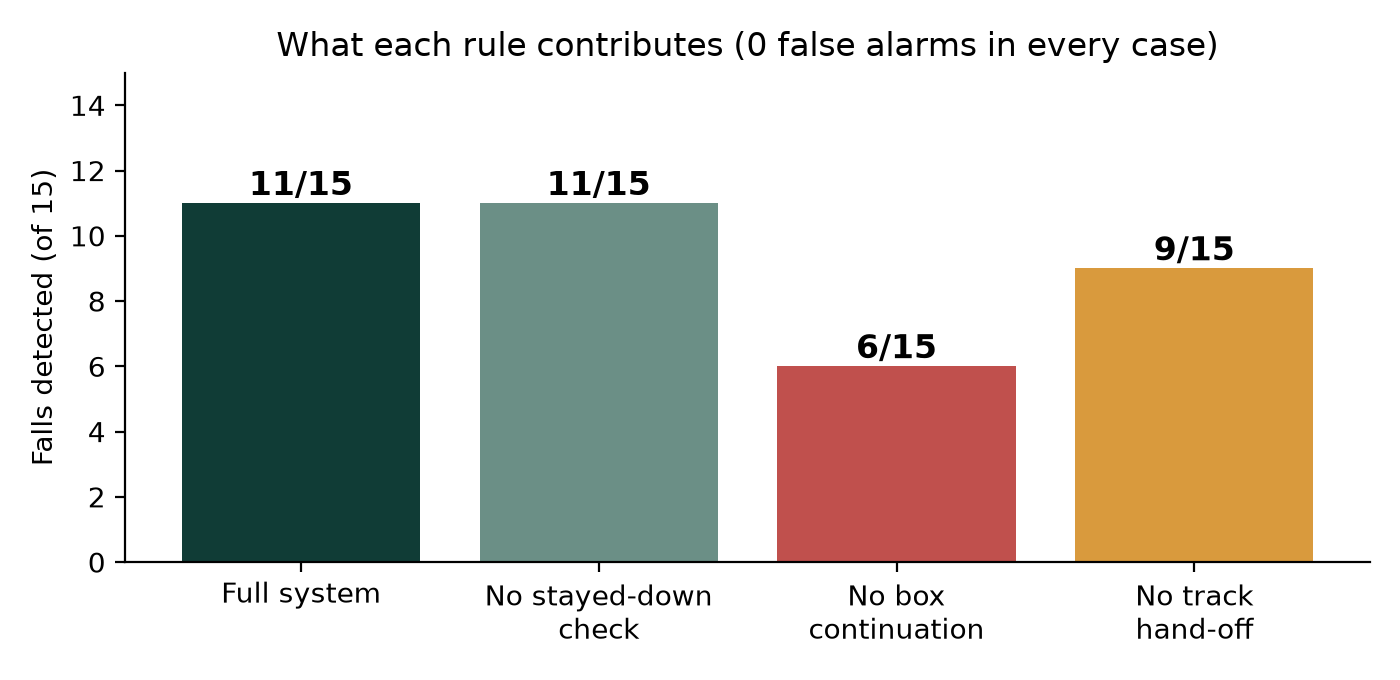
\includegraphics[width=\linewidth]{ablation.png}
\column{0.4\textwidth}
\begin{itemize}\setlength\itemsep{1em}
  \item \textbf{Box continuation} matters most
  \item Alert in about \textbf{4.4 s}
  \item Waiting longer = slower, not safer here
  \item Small dataset: indicative only
\end{itemize}
\end{columns}
\end{frame}

% 11 --------------------------------------------------------------------------------------------
\begin{frame}{Conclusion and next steps}
\begin{columns}[c]
\column{0.5\textwidth}
\textbf{Done}
\begin{itemize}\setlength\itemsep{0.6em}
  \item Ordinary cameras $\to$ active safety monitor
  \item More falls caught, no false alarms
  \item Instant alerts, data stays local
\end{itemize}
\column{0.5\textwidth}
\textbf{Next}
\begin{itemize}\setlength\itemsep{0.6em}
  \item Learn falls from data, not rules
  \item ``Lying too long'' alert
  \item Larger tests, anti-spoofing
\end{itemize}
\end{columns}
\vspace{2.2em}
\centering
{\LARGE\bfseries\color{sentry} Thank you $\cdot$ Questions?}\\[0.6em]
\small\url{github.com/sploitengineer/SentryCare}
\end{frame}

\end{document}
